\documentclass[a4paper,11pt]{article}

% Packages
\usepackage[utf8]{inputenc}
\usepackage[T1]{fontenc}
\usepackage{lmodern}
\usepackage{amsmath, amssymb}
\usepackage{graphicx}
\usepackage{hyperref}
\hypersetup{
    colorlinks=true,
    linkcolor=blue,
    citecolor=black,
    filecolor=black,
    urlcolor=black
}
\usepackage{cleveref}
\usepackage{geometry}
\usepackage{fancyhdr}

% Page layout
\geometry{a4paper, margin=1in}
\pagestyle{fancy}
\fancyhf{}
\fancyhead[L]{TDT4260 Datamaskinarkitektur}
\fancyhead[R]{\thepage}

% Title
\title{TDT4260 Datamaskinarkitektur}
\author{Kristian Gøystdal \\ \\ Username: Kristiangoystdal}
\date{\today}

\begin{document}

\maketitle

The graphs below show the execution time and energy-delay product (EDP) for the different optimizations done on the blur algorithm. All of the values shown in \autoref{fig:time} and \autoref{fig:edp} are from the CMB site, as the VM was not functional.
As shown, the best attempt has a time of $4.06$ seconds and an EDP of $73.74$ J. This is after all the optimizations mentioned below have been applied.


\begin{figure}[h]
  \centering
  \begin{minipage}{0.45\textwidth}
    \centering
    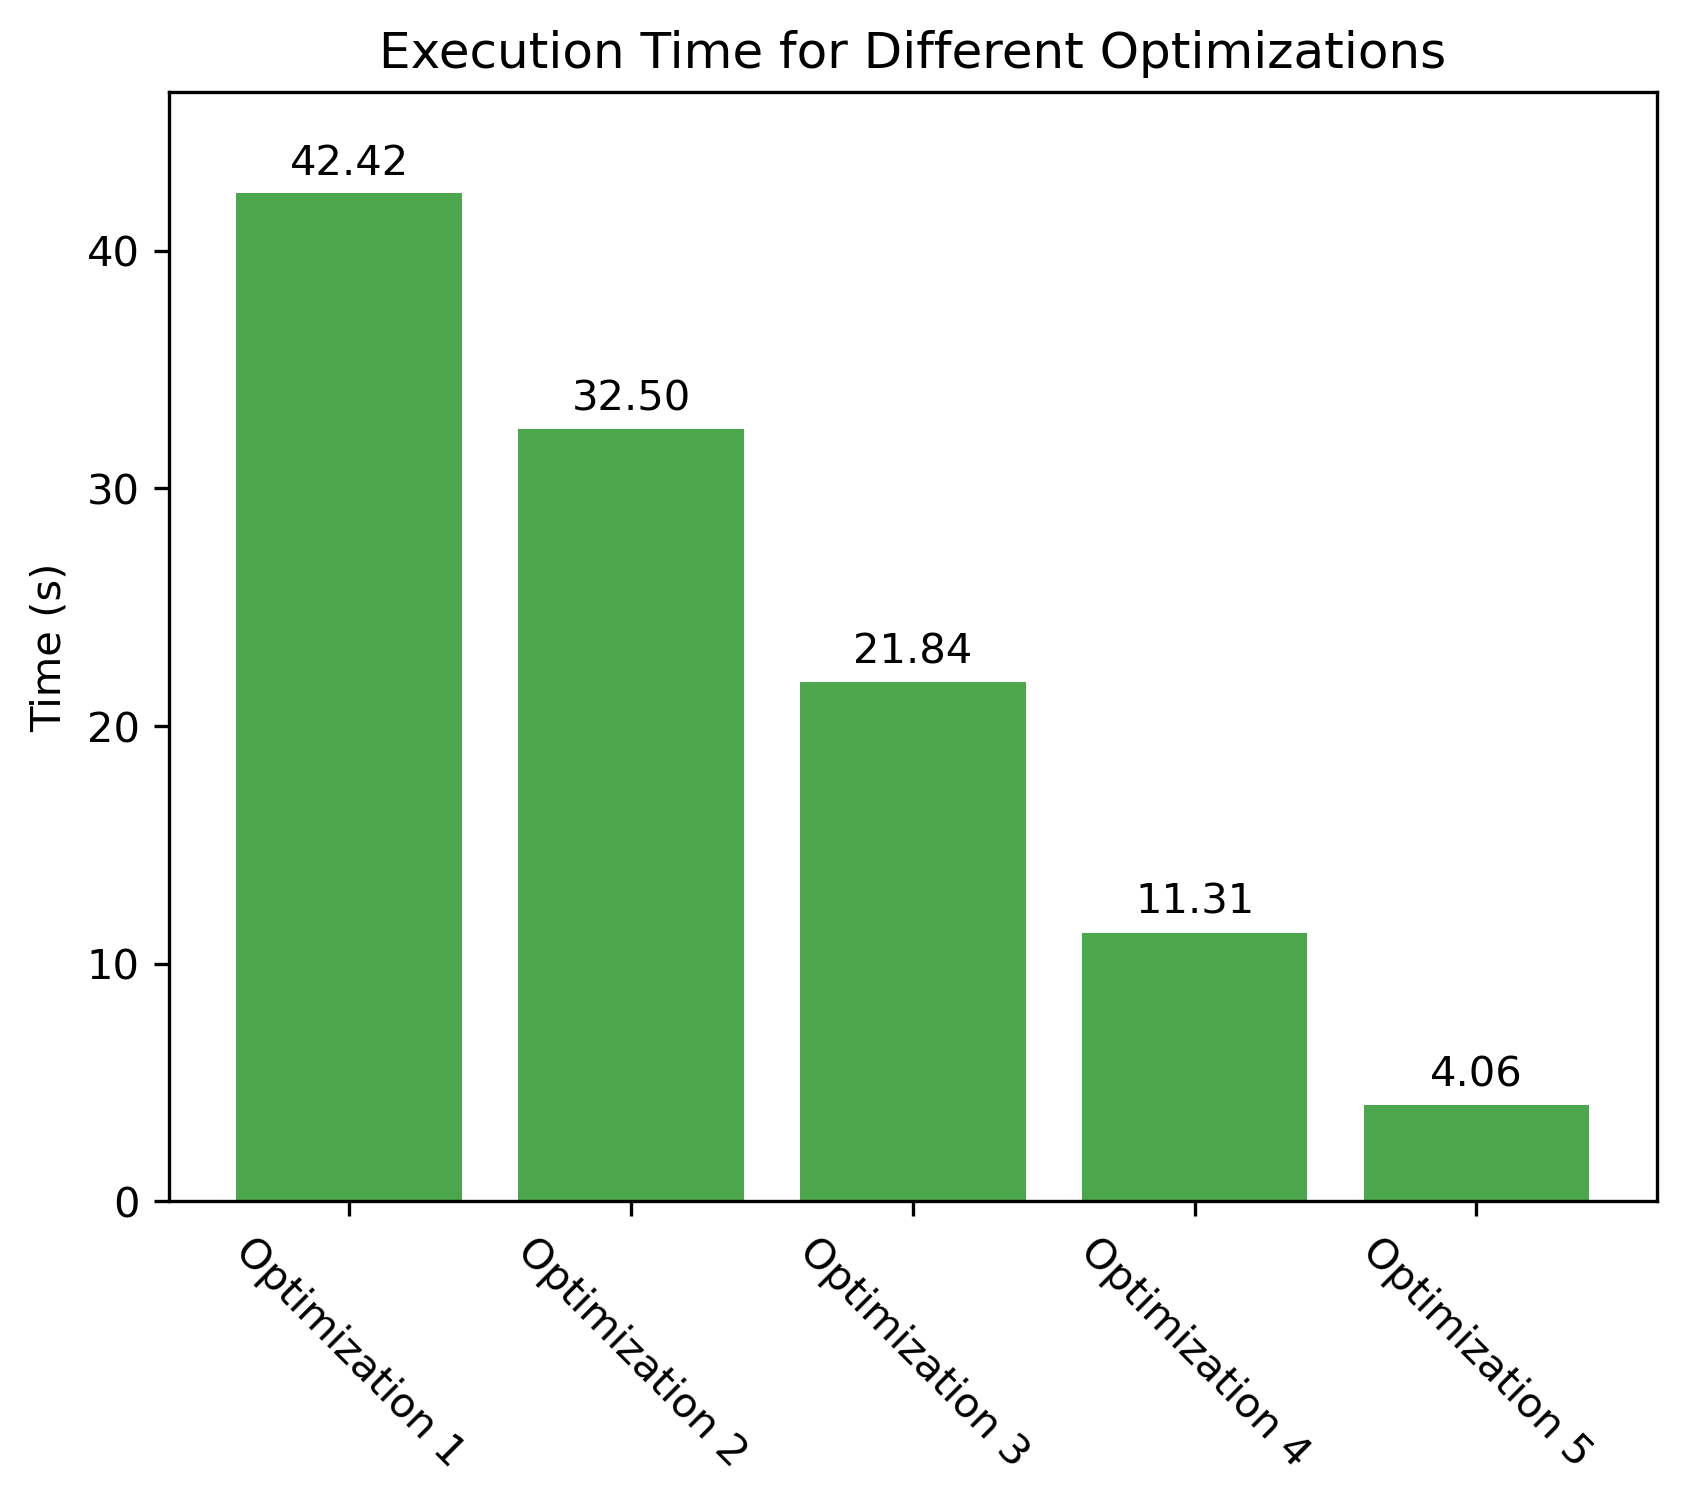
\includegraphics[width=\textwidth]{Time_plot.png}
    \caption{Execution time for the different optimizations done}
    \label{fig:time}
  \end{minipage}
  \hfill
  \begin{minipage}{0.45\textwidth}
    \centering
    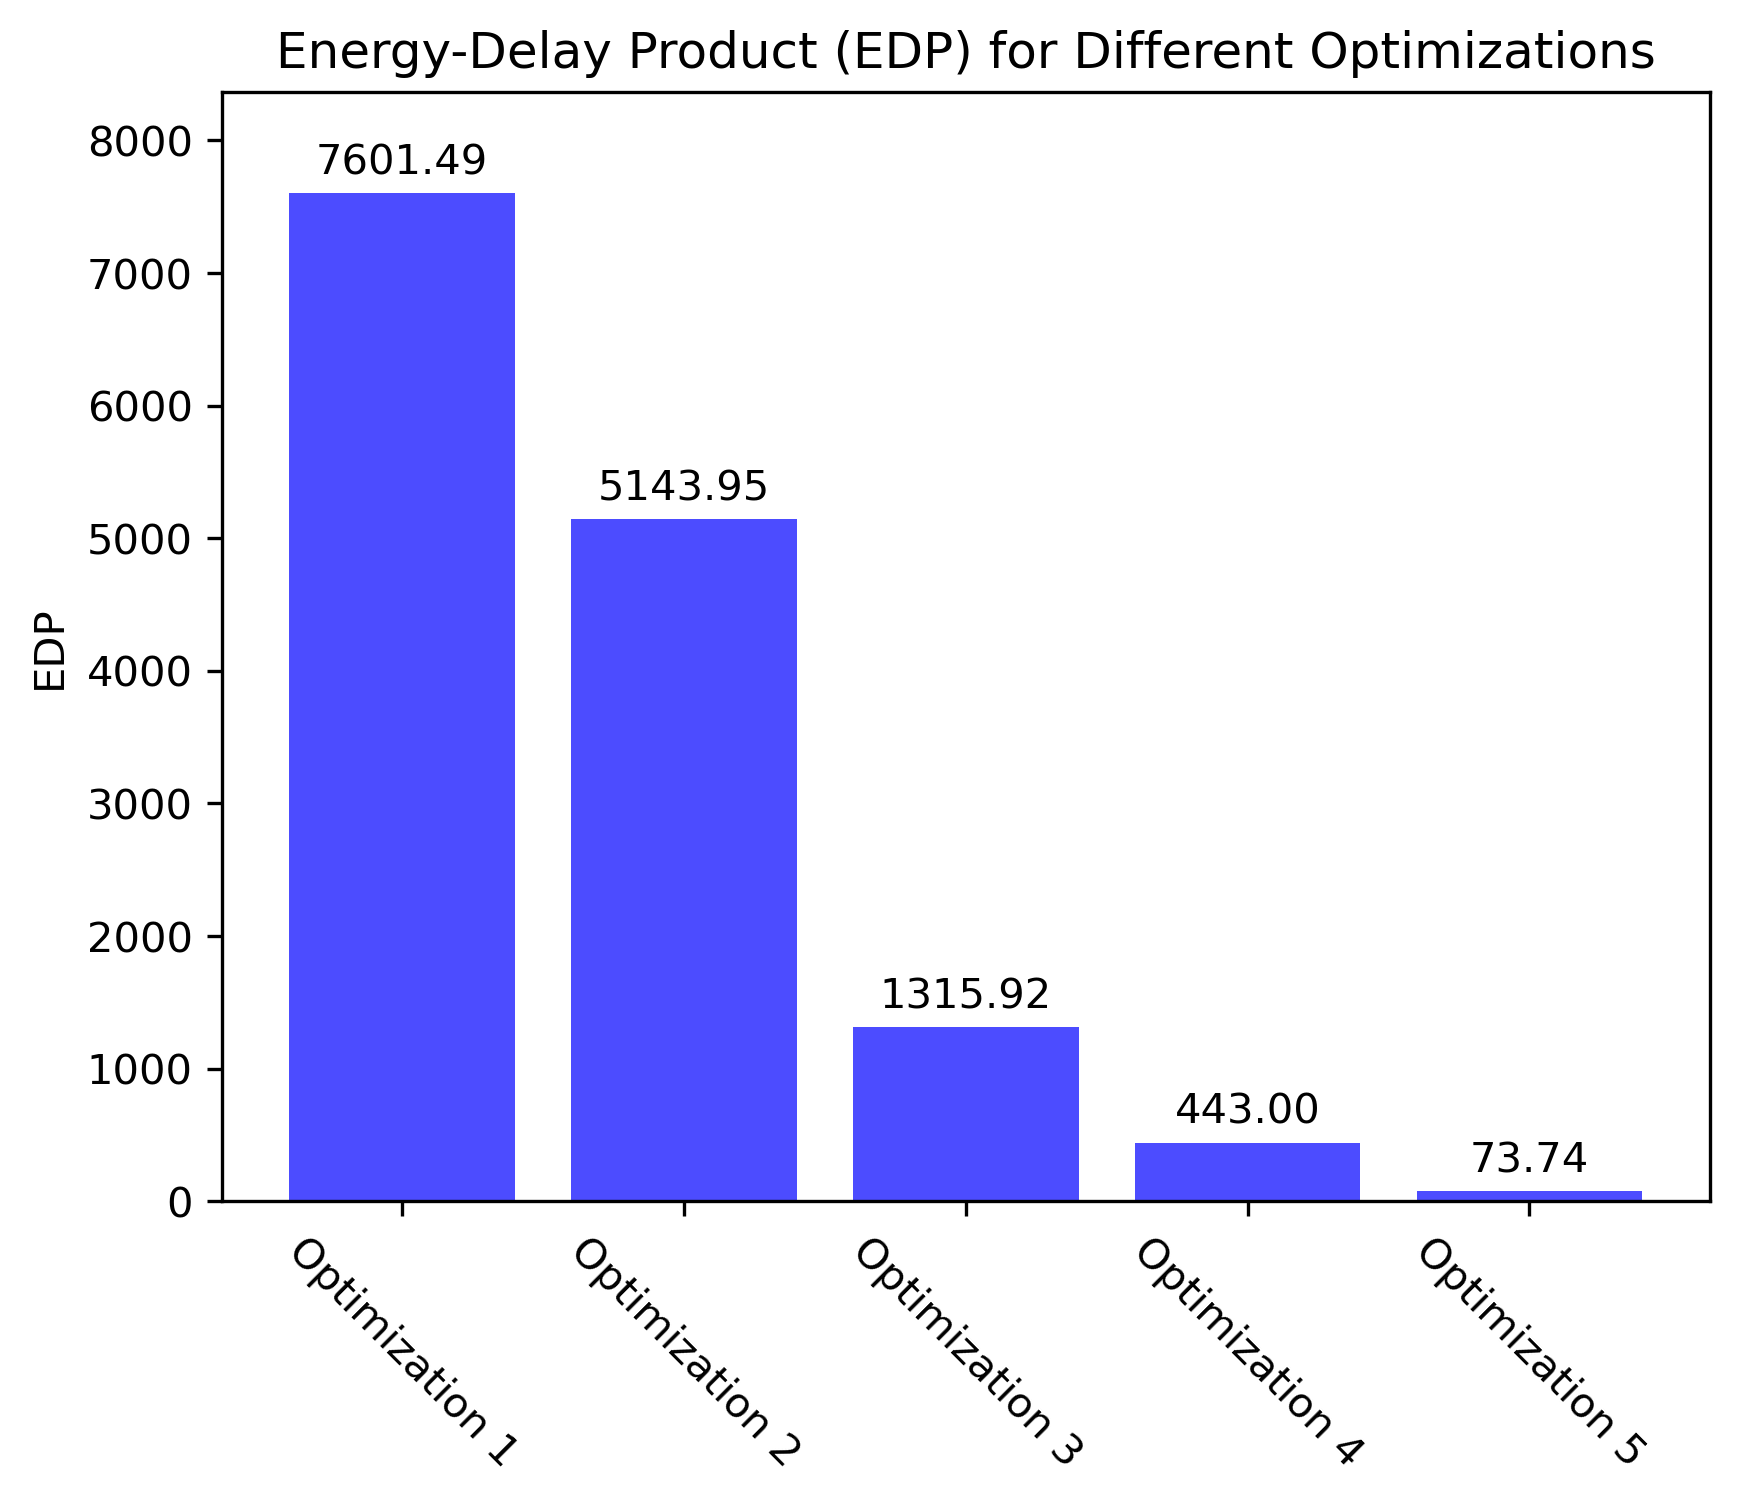
\includegraphics[width=\textwidth]{EDP_plot.png}
    \caption{EDP for the different optimizations done}
    \label{fig:edp}
  \end{minipage}
\end{figure}


\section*{Optimization 1 - Improved Memory Access Pattern} 
This optimization focuses on improving the performance of matrix operations, which are common in many applications.
The base algorithm for blur iterates over the image by accessing the x-axis first, which is not cache-friendly.
The optimized algorithm iterates over the y-axis first, which improves the performance by reducing the number of cache accesses. 

\section*{Optimization 2 - OpenMP Loop Parallelization}
The next optimization uses parallelization from OpenMP to improve performance. By parallelizing the outer loop, we can take advantage of multiple cores in the CPU and run multiple iterations of the loop simultaneously. This can significantly reduce the execution time for large matrices.

\section*{Optimization 3 - Algorithmic Complexity Reduction (2D → 1D)}
The next optimization done is a convertion from the 2D blur algorithm to a 1D blur algorithm. The 2D algorithm have to run $n^2$ iterations, while the 1D algorithm only have to run $n$ iterations for each direction. By running the 1D algorithm for horizontal first, and then the vertical, the number of iterations are significantly reduced from $n^2$ to $2n$.


\section*{Optimization 4 - Combined Color Channel Processing}
This optimization focuses on the way the different colors are handled in the blur algorithm. The colors are now handled all at the same time instead of having to execute one blur operation for each color. 

\section*{Optimization 5 - Parallel Processing Across Image Sizes}
The final optimization is to parallelize the operations done on the different image sizes. The different image sizes are independent of each other, and can be run in parallel. 


\section*{AI Decleration}
No AI tools were used in producing this report. 

\end{document}